%%
%% User Guide
%%

%%%%%%%%%%%%%%%%%%%%%%%%%%%%%%%%%%%%%%%%%%%%%%%%%%%%%%%%%%%%%%%%%%%%%%%%%%%%%%%%
\chapter{User Guide} \label{chapter:user_guide}
%%%%%%%%%%%%%%%%%%%%%%%%%%%%%%%%%%%%%%%%%%%%%%%%%%%%%%%%%%%%%%%%%%%%%%%%%%%%%%%%


%%%%%%%%%%%%%%%%%%%%%%%%%%%%%%%%%%%%%%%%%%%%%%%%%%%%%%%%%%%%%%%%%%%%%%%%%%%%%%%%
\section{\qsimavr User Guide}
%%%%%%%%%%%%%%%%%%%%%%%%%%%%%%%%%%%%%%%%%%%%%%%%%%%%%%%%%%%%%%%%%%%%%%%%%%%%%%%%

Within this guide, we will assume the use of firmware compiled for the
\verb|atmega1280| with a frequency of 16 \ac{MHz}\footnote{
%
These are the default settings.
%
}. After starting \qsimavr, you are presented with a screen which should look
somewhat similar to figure \ref{fig:qsimavr}.

\begin{figure}[ht]
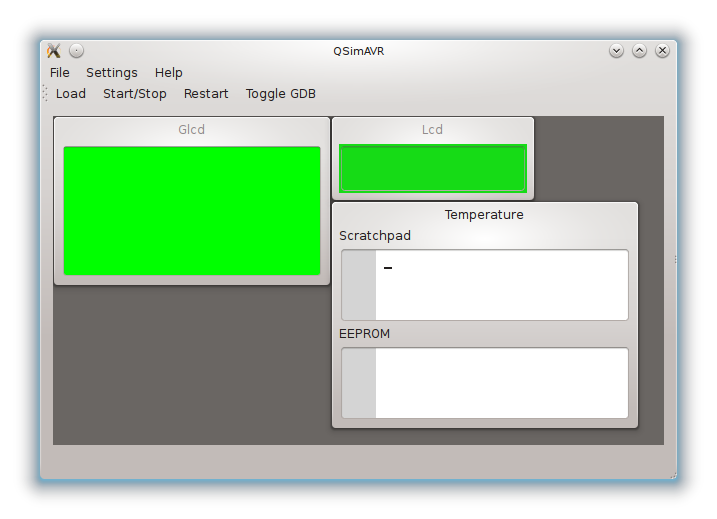
\includegraphics[width=\textwidth]{images/qsimavr}
\caption{\qsimavr}
\label{fig:qsimavr}
\end{figure}

Trace and error output, as well as \simavr messages are printed directly to the
console. \ac{VCD} files are saved into the current working directory.

Loaded components can be configured in the \emph{Settings} menu. Currently,
possible options include enabling or disabling a component and toggling \ac{VCD}
traces.

A firmware file may be loaded by either pressing \emph{Load} in the toolbar,
selecting \emph{Load Firmware...} in the \emph{File} menu, or clicking on one of
the recently loaded files listed in the \emph{File} menu. Simulation starts
automatically once the firmware file has been loaded successfully.

The current simulation state is displayed in the lower left of the status bar
once a firmware file has been loaded.

For debugging (also see \ref{section:debugging}), \ac{GDB} support must be enabled
by clicking the \emph{Toggle \ac{GDB}} button in the toolbar. If a simulation is
currently in progress, execution is halted (note the change in simulation state);
otherwise the \ac{CPU} will be paused once the next firmware file has been loaded
or the simulation is restarted.

Once running, it is possible to pause and unpause the simulation by pressing the
\emph{Start/Stop} button in the toolbar, or restarting it by pressing
\emph{Restart}.

The components are all fairly self-explanatory to use. The \ac{EEPROM}, \ac{RTC}
and temperature sensor display their memory contents in a hex editor which
can also be used to alter their state; the \ac{GLCD} acts as a touchscreen on
mouse presses. The \ac{LED} buttons can of course be clicked to interact with the
\ac{AVR} core\footnote{
%
Because of the large number of connected \acp{IRQ}, it is sometimes a good idea
to disable the \ac{LED} buttons component when running a firmware with a high
frequency of port traffic.
%
}.


%%%%%%%%%%%%%%%%%%%%%%%%%%%%%%%%%%%%%%%%%%%%%%%%%%%%%%%%%%%%%%%%%%%%%%%%%%%%%%%%
\section{Debugging with \simavr and \ac{GDB}} \label{section:debugging}
%%%%%%%%%%%%%%%%%%%%%%%%%%%%%%%%%%%%%%%%%%%%%%%%%%%%%%%%%%%%%%%%%%%%%%%%%%%%%%%%

As discussed in section \ref{section:gdb_support}, \simavr supports \ac{GDB}
through the Remote Serial Protocol, which allows us to debug \ac{AVR} programs
locally or even from a remote location. Debugging is enabled in \qsimavr by
clicking on the \emph{Toggle \ac{GDB}} button in the toolbar. Further steps
are exactly the same as when starting \simavr with the \verb|-g| flag.

Let's walk through a debugging session of a short example program\footnote{
%
This is the interrupt \& callback demo of the Microcontroller course at the
\ac{TU} Vienna. The source code is  also available at \url{http://ti.tuwien.ac.at/ecs/teaching/courses/mclu/manuals/demo-programs/c-interrupt-demo/at_download/file} (accessed 2012-08-31).
%
}, reproduced
in full here:

\begin{lstlisting}
/**
    This is the C interrupt callback demo.

    Enable the LEDs for port A.
    Whenever INT7 or INT6 is pressed the counting
    mode changes from increasing to decreasing and vice versa.
*/

#define F_CPU       (16000000UL)

#include <avr/io.h>
#include <avr/sleep.h>
#include <avr/interrupt.h>

#ifndef NULL
#define NULL    ((void *) 0)
#endif
#ifndef TRUE
#define TRUE    (0 == 0)
#endif
#ifndef FALSE
#define FALSE   (!TRUE)
#endif

/* prototypes */
static uint8_t increment(const uint8_t counter);
static uint8_t decrement(const uint8_t counter);
static void setCallback(uint8_t (*_interrupt)(const uint8_t counter));
static void callCallback(volatile uint8_t *counter);

/* variables */
static uint8_t (*interrupt)(const uint8_t counter);
static volatile uint8_t isFallingEdge, click;

int main(void)
{
    /* initialize variables */
    setCallback(&increment);
    isFallingEdge = TRUE;
    click = FALSE;

    /* Initialize LEDs. */
    DDRA = 0xFF;
    PORTA = 0x00;

    /* Set up interrupts */
    DDRE  &= ~((1<<PE6) | (1<<PE7));
    PORTE |= (1<<PE6)   | (1<<PE7);
    EICRB = (EICRB & ~((1<<ISC60) | (1<<ISC70))) | (1<<ISC61) | (1<<ISC71);
    EIMSK |= (1<<INT6)  | (1<<INT7);

    /* Set up timer interrupt */
    TCCR1A &= ~(_BV(COM1A1) | _BV(COM1A0) | _BV(COM1B1) | _BV(COM1B0) | _BV(COM1C1) | _BV(COM1C0) | _BV(WGM11) | _BV(WGM10));
    TCCR1B &= ~(_BV(ICNC1) | _BV(WGM13) | _BV(ICES1) | _BV(CS12) | _BV(CS11) | _BV(CS10));
    OCR1A = ((250 * F_CPU) / (64 * 1000U)) - 1;
    TIMSK1 |= _BV(OCIE1A);
    TCCR1B |= _BV(CS11) | _BV(CS10) | _BV(WGM12);

    sei();

    set_sleep_mode(SLEEP_MODE_IDLE);
    sleep_enable();

    while(TRUE)
    {
        /* Set CPU to sleep mode. */
        sleep_cpu();
    }
    return 0;
}

/* helper functions */
static uint8_t decrement(const uint8_t counter)
{
    return counter - 1;
}

static uint8_t increment(const uint8_t counter)
{
    return counter + 1;
}

static void setCallback(uint8_t (*_interrupt)(const uint8_t counter))
{
    interrupt = _interrupt;
}

static void callCallback(volatile uint8_t *counter)
{
    if(interrupt != NULL)
    {
        *counter = (*interrupt)(*counter);
    }
}

/* interrupts */
ISR(TIMER1_COMPA_vect, ISR_BLOCK)           /* Blocking timer interrupt */
{
    static volatile uint8_t counter = 0;

    click = FALSE;
    callCallback(&counter);
    PORTA = counter;
}

ISR(INT7_vect, ISR_NOBLOCK)                 /* Non blocking interrupt on PE7 */
{
    if(!click)
    {
        if(isFallingEdge)
            setCallback(&decrement);
        else
            setCallback(&increment);

        isFallingEdge = !isFallingEdge;
    }
    click = TRUE;
}

ISR(INT6_vect, ISR_ALIASOF(INT7_vect));       /* Alias for PE6 to do the same as on PE7 */
\end{lstlisting}

This program executes a callback function once per timer interrupt, which either
increases or decreases the value displayed on the \verb|PORTA| \acp{LED}. The selected callback
can be switched by triggering \lstinline|INT7| or \lstinline|INT6|, which correspond
to the buttons on \verb|PORTE6| and \verb|PORTE7|.

We will begin by testing \simavr's \ac{GDB} passive mode, which is triggered on
invalid memory accesses, such as trying to read from \lstinline|RAMEND + 1|:

\begin{lstlisting}
diff --git a/main.c b/main.c
index 5cc85f9..2d04541 100644
--- a/main.c
+++ b/main.c
@@ -41,7 +41,7 @@ int main(void)

     /* Initialize LEDs. */
     DDRA = 0xFF;
-    PORTA = 0x00;
+    PORTA = *((uint8_t *)RAMEND + 1);

     /* Set up interrupts */
     DDRE  &= ~((1<<PE6) | (1<<PE7));
\end{lstlisting}

Compile this program, making sure to include debug symbols by passing the \verb|-g|
flag:

\begin{verbatim}
avr-gcc -mmcu=atmega1280 -Wall -Wstrict-prototypes -Os
    -frename-registers -fshort-enums -fpack-struct -g
    -c -o main.o main.c
avr-gcc -mmcu=atmega1280 -Wl,-u,vfprintf -lprintf_min
    -o main.elf main.o
\end{verbatim}

Load the firmware into \qsimavr. As soon as execution hits the invalid memory
access, an error message is printed, and \ac{GDB} is automatically set up to listen
on port 1234:

\begin{verbatim}
CORE: *** Invalid read address PC=0498 SP=21fd O=4091
    Address 2200 out of ram (21ff)
avr_sadly_crashed
\end{verbatim}

We can now connect \ac{GDB}\footnote{
%
Make sure you are using the \ac{AVR} version of \ac{GDB}, usually called \emph{avr-gdb}.
%
} to the simulation by executing \verb|target remote localhost:1234|. Debugging symbols
are then loaded by pointing \ac{GDB} towards the \ac{ELF} file with \verb|file main.elf|.
We can now start digging around for the error; for example, to see a disassembly
of area around the current \ac{PC}, type in \verb|disassemble|. To retrieve the
values of all registers, type \verb|info registers|. A backtrace can be created
by typing \verb|backtrace|.

\begin{verbatim}
(gdb) target remote localhost:1234
Remote debugging using localhost:1234
0x0000049c in ?? ()
(gdb) file main.elf
A program is being debugged already.
Are you sure you want to change the file? (y or n) y
Reading symbols from main.elf...done.
(gdb) disassemble
Dump of assembler code for function main:

   [...]

   0x00000498 <+26>:    lds     r20, 0x2200
=> 0x0000049c <+30>:    out     0x02, r20       ; 2
   0x0000049e <+32>:    in      r21, 0x0d       ; 13

   [...]

End of assembler dump.
(gdb) info registers

    [...]

r29            0x21     33
r30            0x0      0
r31            0x0      0
SREG           0x2      2
SP             0x8021fd 0x8021fd
PC2            0x49e    1182
pc             0x49e    0x49e <main+32>
(gdb) bt
#0  main () at main.c:47
\end{verbatim}

You can either experiment further with \acp{GDB} commands, read through the
inline help (type \verb|help|), or quit \ac{GDB} by typing \verb|quit|.
\simavr's passive mode is very useful in situations where a program crashes
unexpectedly.

Let'd do some more deliberate debugging. Fix your program by reverting the
invalid memory reference we inserted above, make sure \ac{GDB} support is
switched on in \qsimavr, and load the newly compiled firmware. You already know
how to attach \ac{GDB} and load debugging symbols:

\begin{verbatim}
(gdb) target remote localhost:1234
(gdb) file main.elf
\end{verbatim}

Say we're interested in the \lstinline|increment| function, and we'd like to
examine every execution of it. Settings a breakpoint will halt simulation
every time that function is called. We can either set breakpoints by
function names, or by file name and line numbers:

\begin{verbatim}
(gdb) break increment
Breakpoint 1 at 0x128: file main.c, line 81.
(gdb) break main.c:81
Note: breakpoint 1 also set at pc 0x128.
Breakpoint 2 at 0x128: file main.c, line 81.
\end{verbatim}

Breakpoints can be deleted by using the \verb|delete| command:

\begin{verbatim}
(gdb) delete 2
\end{verbatim}

Now, continue running the simulation with the \verb|continue| command.
As soon as \lstinline|increment| is called for the first time,
simulation pauses and control is returned to \ac{GDB}:

\begin{verbatim}
(gdb) continue
Continuing.

Breakpoint 1, increment (counter=0 '\000') at main.c:81
81      }
\end{verbatim}

The current location within the source code can be printed by using the \verb|list|
command. We can also examine (and even change) variable values with the \verb|print|
and \verb|list| commands. It is even possible to call functions on demand with
\verb|call|:

\begin{verbatim}
(gdb) print counter
$1 = 0 '\000'
(gdb) set counter = 42
(gdb) print counter
$2 = 42 '*'
(gdb) call decrement(counter)
$3 = 41 ')'
\end{verbatim}

What if you were actually interested in all places in which the counter value
is accessed instead of specific locations in your program? This kind of monitoring
is also possible using \ac{GDB} watchpoints, which alert \ac{GDB} whenever the
value of an \ac{SRAM} location changes:

\begin{verbatim}
(gdb) delete
Delete all breakpoints? (y or n) y
(gdb) watch counter
Watchpoint 3: counter
(gdb) continue
Continuing.
Watchpoint 3: counter

Old value = 42 '*'
New value = 43 '+'
0x0000012a in increment (counter=43 '+') at main.c:81
81      }
\end{verbatim}

This concludes our short tour of debugging \ac{AVR} programs with \qsimavr and
\ac{GDB}. For further details, consult the \ac{GDB} documentation \cite{gdb} or
one of the innumerable \ac{GDB} tutorials which can be found on the net\footnote{
%
A good one is RMS' gdb Debugger Tutorial at \url{http://www.unknownroad.com/rtfm/gdbtut/gdbtoc.html}.
%
}.
